\section{Methods}

\subsection{Linear Programming Framework}

Linear programming (LP) provides a mathematical framework for solving
optimization and feasibility problems subject to linear constraints. In the
present work, LP is used to reformulate activation screening as a feasibility
problem in composition space. Rather than generating candidate alloy
compositions and subsequently evaluating whether they satisfy prescribed
activation criteria, the activation criteria are expressed directly as
constraints on alloy composition. The set of compositions satisfying all
constraints defines a feasible region within the atomic-fraction simplex. This
reformulation shifts the focus from evaluating individual compositions to
constructing and exploring the admissible region of composition space itself.

The applicability of LP to the present problem arises from the linear dependence
of \textsc{FLARE} activation responses on alloy composition. Because the FLARE alloy
response is linear in composition, its response coefficients can be assembled
directly into a system of linear inequalities in composition space, the
activation criteria become LP constraints, and LP is used to define the polytope
that bounds the feasible region. Once the polytope is constructed, its geometry is
characterized analytically through vertex enumeration, and feasible alloy
compositions are obtained by enumerating the 5~at.\% grid points contained in the polytope. The
framework therefore replaces conventional generate-and-filter screening with a
constraint-first methodology that directly identifies compositions satisfying
the prescribed activation requirements. Figure~\ref{fig:lp-workflow} contrasts
the two workflows.

\begin{figure*}[!t]
    \centering
    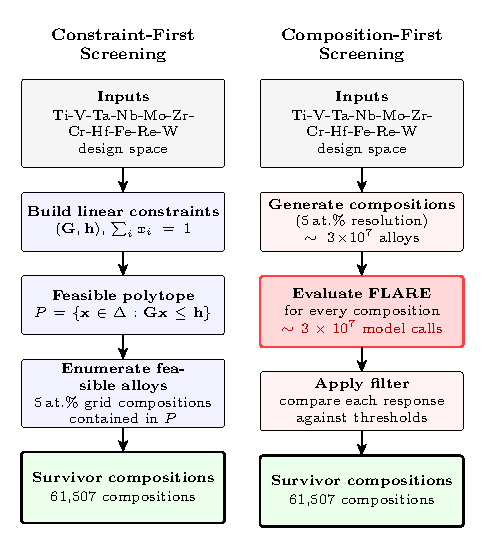
\includegraphics[width=0.7\textwidth]{./figures/lp_workflow.pdf}
    \caption{Side-by-side comparison of constraint-first screening (left,
    proposed in this work) and composition-first screening (right, the
    conventional generate-and-filter workflow). The constraint-first path
    assembles the activation criteria into the linear constraint system
    \((\mathbf{G},\mathbf{h})\), defines the feasible polytope
    \(P=\{\mathbf{x}\in\Delta:\mathbf{G}\mathbf{x}\le\mathbf{h}\}\), and
    enumerates the 5\,at.\% grid compositions contained in \(P\). The
    composition-first path instead generates all \(\sim 3{\times}10^{7}\) grid
    compositions, evaluates the FLARE response model for each, and filters the
    results against the screening thresholds. Both paths recover the identical
    feasible set: \(61{,}507\) compositions summed across the two reference
    screens, comprising \(61{,}303\) distinct compositions once the \(204\)
    compositions feasible under both references are counted once.}
    \label{fig:lp-workflow}
\end{figure*}

\subsubsection{Design Domain and Activation Responses}

The alloy design domain considered in this work consists of the eleven-element
refractory system comprising \ch{Ti-V-Ta-Nb-Mo-Zr-Cr-Hf-Fe-Re-W}. An
alloy is represented by its atomic-fraction vector
\(\mathbf{x}=(x_1,\ldots,x_N)\) with \(N=11\), where \(x_i\) is the atomic
fraction of element \(i\). Physically admissible compositions lie on the
standard \((N-1)\)-simplex
\(\Delta = \{\mathbf{x}\in\mathbb{R}^{N} : \sum_i x_i = 1,\; x_i \ge 0\}\). The
discrete design domain is the regular 5~at.\% grid on \(\Delta\), i.e., the set
of compositions whose fractions are integer multiples of \(0.05\). On an
eleven-element simplex, this grid contains approximately \(3\times10^{7}\)
compositions, illustrating the computational burden associated with conventional
generate-and-filter screening.

Candidate alloys are screened based on their neutron-activation response using
the FLARE reduced-order model~\cite{flare}. FLARE computes each activation response of an
alloy as a composition-weighted sum of pre-tabulated per-element coefficients,
so that every response is linear in alloy composition, in contrast to full
inventory simulations that evaluate each composition individually~\cite{sublet2017fispact}. Responses are evaluated
at a neutron flux of \(8.0\times10^{13}~\mathrm{n~cm^{-2}~s^{-1}}\), an
irradiation time of 2~years, and the decay times associated with each screening
criterion. For fixed flux, irradiation time, and decay time, responses are
averaged over the available neutron spectra.

Screening is performed using five activation responses: gas production
\(M_{\mathrm{GAS}}\), total heat output \(HT_T\), and displacement damage
\(DPA\) at a decay time of approximately 1~s, together with contact dose rate
\(DOSE\) at decay times of 1~month and 100~years. Each response is assembled
from its per-element contributions on the appropriate extensive basis: by
weight fraction for the mass-extensive responses
\((M_{\mathrm{GAS}}, HT_T, DOSE)\) and by atomic fraction for the atom-extensive
response \((DPA)\). This distinction determines the exact form of the linear
constraints constructed in Section~\ref{sec:activation-constraints}. Activation thresholds are defined
relative to tungsten (W) and EUROFER97 reference response vectors. Together with
the FLARE alloy-response coefficients, these reference vectors form the basis
from which the LP constraint system is constructed in the following section.


\subsubsection{Activation Criteria as Linear Constraints}
\label{sec:activation-constraints}

The activation screening criteria are imposed directly on the FLARE response
model and reformulated as linear inequalities in composition space. The linear
coefficients of the FLARE alloy response model are collected in the response
matrix \(\mathbf{A}\in\mathbb{R}^{R\times N}\), where \(A_{r,i}\) is the linear
coefficient of element \(i\) in response \(r\), with \(R=5\) screening responses
and \(N=11\) elements. Each screening threshold is defined relative to a reference
alloy as \(\tau_r = \phi\, b_r\), where
\(\mathbf{b}=(b_1,\ldots,b_R)\) is the reference response vector, taken as
either tungsten \((\mathbf{b}_W)\) or EUROFER97 \((\mathbf{b}_E)\), and
\(\phi = 10\) is the threshold multiplier.

Each criterion is then expressed as a linear inequality in the atomic-fraction
vector \(\mathbf{x}\). The atom-extensive response \(DPA\) combines directly by
atomic fraction and is therefore already linear in \(\mathbf{x}\),

\begin{equation}
\sum_i x_i A_{r,i} \le \phi\, b_r .
\label{eq:atom_constraint}
\end{equation}

The mass-extensive responses \((M_{\mathrm{GAS}}, HT_T, DOSE)\) combine by
weight fraction,

\begin{equation}
w_i = \frac{x_i M_i}{\sum_j x_j M_j} ,
\label{eq:weight_fraction}
\end{equation}

where \(M_i\) is the atomic mass of element \(i\). Substituting
Eq.~\eqref{eq:weight_fraction} into the natural constraint
\(\sum_i w_i A_{r,i} \le \phi b_r\) introduces the composition-dependent
denominator \(\sum_j x_j M_j\), making the expression nonlinear in
\(\mathbf{x}\). Because this denominator is strictly positive on the simplex,
multiplying through by it preserves the inequality while eliminating the
nonlinearity, yielding the equivalent linear form

\begin{equation}
\sum_i x_i M_i \left(A_{r,i} - \phi\, b_r\right) \le 0 .
\label{eq:mass_constraint}
\end{equation}

Equations~\eqref{eq:atom_constraint} and~\eqref{eq:mass_constraint} are both
linear in \(\mathbf{x}\). Stacking all \(R\) screening criteria together with
the box bounds \(0\le x_i \le 1\) yields the linear inequality system
\(\mathbf{G}\mathbf{x}\le\mathbf{h}\), in which the \(DPA\) row contributes the
coefficients \(A_{r,i}\) with right-hand side \(\phi b_r\), while each
mass-extensive response contributes the transformed coefficients
\(M_i(A_{r,i}-\phi b_r)\) with right-hand side zero. Together with the simplex
equality \(\sum_i x_i = 1\), the constraint system defines the complete LP feasibility problem. The corresponding solution set forms a convex feasible polytope in composition space, which provides an analytical representation of the activation-feasible design region.


\subsubsection{Feasible Polytope and Alloy Enumeration}

The linear constraint system \(\mathbf{G}\mathbf{x}\le\mathbf{h}\), together with
the simplex equality \(\sum_i x_i=1\), defines the set of all compositions
satisfying the activation criteria as the convex polytope
\[
P=\{\mathbf{x}\in\Delta:\mathbf{G}\mathbf{x}\le\mathbf{h}\}.
\]
The rows of \(\mathbf{G}\) and \(\mathbf{h}\) encode the FLARE response
coefficients and the screening thresholds, so compositions inside \(P\) satisfy
every criterion while those outside violate at least one. The vertices of \(P\)
were obtained through active-constraint enumeration. A vertex is the composition
fixed uniquely by the simplex equality together with \(N-1\) active constraints obtained by solving

\medskip
\begin{equation}
\begin{bmatrix} \mathbf{1}^{\top} \\ \mathbf{G}_{\mathcal{A}} \end{bmatrix}
\mathbf{x}
=
\begin{bmatrix} 1 \\ \mathbf{h}_{\mathcal{A}} \end{bmatrix} ,
\label{eq:vertex_system}
\end{equation}
\medskip


for the active set \(\mathcal{A}\), with \(\mathbf{G}_{\mathcal{A}}\) and
\(\mathbf{h}_{\mathcal{A}}\) the active constraint rows; solutions were retained
only if they satisfied the complete system.

To obtain discrete alloy candidates from the continuous feasible region, the
interior of \(P\) was discretized on a \(5\)~at.\% composition grid, and all grid
points within \(P\) were enumerated exactly. Rather than generating the full grid
and testing each point for membership, a depth-first recursion enumerates the
feasible points directly. At depth \(p\), with elements \(1,\dots,p-1\) fixed, two
linear programs determine the minimum and maximum values of the next fraction
\(x_p\) for which a feasible completion of the remaining composition exists,

\medskip
\begin{equation}
\begin{aligned}
x_p^{\min},\,x_p^{\max}
&=
\min,\max
\left\{
\begin{array}{l}
x_p : \mathbf{G}'\mathbf{x}' \le \mathbf{s},\\[4pt]
\mathbf{1}^{\top}\mathbf{x}'=\rho,\\
0 \le \mathbf{x}' \le \rho
\end{array}
\right\}
\end{aligned}
\label{eq:interval_lp}
\end{equation}
\medskip


where \(\mathbf{s}\) is the residual constraint slack after accounting for the
previously specified composition variables and \(\rho\) is the remaining
composition fraction. Solving Eq.~(\ref{eq:interval_lp}) determines the feasible
bounds of the next composition variable within the remaining composition space,
and repeated application throughout the recursion yields every \(5\)~at.\% grid
composition contained in \(P\). The enumeration returned the identical feasible
set, the same compositions, as a conventional generate-and-filter workflow
(Section~\ref{sec:results}), while avoiding explicit evaluation of every
candidate composition.


\subsection{High-Throughput Property Calculations}

Following activation screening, the remaining compositions were assessed using
analytical models of mechanical performance. Because direct experimental
characterization or high-fidelity mechanical simulations are impractical for the
large number of candidate alloys considered in this work, physically motivated
analytical models were employed as first-order estimates of strength and
ductility. These models provide a computationally efficient means of evaluating
strength and ductility descriptors for the candidate compositions in advance of the
subsequent thermodynamic characterization.

\subsubsection{Maresca-Curtin Model as First Approximation for Yield Strength}

The feasible alloy compositions were subsequently evaluated using the Maresca-Curtin (MC) model as a first approximation of alloy yield strength \cite{maresca2020mechanistic}. The model has been successfully employed for the computational screening and design of refractory multi-principal-element alloys \cite{vela2023data}, and the present implementation follows the general methodology adopted in those studies. In this work, the model was used to compute first-order strength descriptors for the candidate compositions prior to thermodynamic characterization.

The MC model is a physics-based framework for body-centered cubic (BCC) random solid solutions that relates alloy strength to the energetics of thermally activated dislocation motion. In this work, the temperature-dependent yield strength was evaluated using the dislocation-glide formulation proposed by Maresca and Curtin.

\vspace{0.5em}

\begin{equation}
\begin{aligned}
\tau_y(T,\dot{\varepsilon})
&= \tau_{y0}
\exp\!\left[
-\frac{1}{0.55}
\left(
\frac{kT}{\Delta E_b}
\ln\!\left(\frac{\dot{\varepsilon}_0}{\dot{\varepsilon}}\right)
\right)^{0.91}
\right]
\end{aligned}
\label{eq:yield_stress}
\end{equation}

\vspace{0.5em}

where $\tau_{y0}$ is the athermal yield strength, $\Delta E_b$ is the activation barrier for dislocation glide, $T$ is the absolute temperature, $\dot{\varepsilon}$ is the applied strain rate, $\dot{\varepsilon}_0$ is the reference strain rate, and $k$ is Boltzmann's constant. The corresponding tensile yield strength was obtained through the appropriate Taylor-factor conversion.

Following the approach of Vela et al.~\cite{vela2023data}, the physical inputs required by the model, including atomic volumes, elastic constants ($C_{11}$, $C_{12}$, and $C_{44}$), shear moduli, and Poisson ratios, were assembled from literature data and combined using the rule of mixtures to approximate the effective properties of each alloy composition.

Yield strengths were evaluated at 25, 600, and $650^{\circ}\mathrm{C}$ using a strain rate of $10^{-3}\,\mathrm{s}^{-1}$. The resulting yield strengths were recorded as mechanical-property descriptors.

\subsubsection{Nimplex Graph Representation of Alloy Spaces}

discuss nimplex here 

\subsubsection{CALPHAD Thermodynamic Calculations}

The feasible alloy compositions were subsequently evaluated using the CALPHAD (CALculation of PHAse Diagrams) method to characterize their thermodynamic stability, phase constitution, melting behavior, and thermophysical properties. CALPHAD has been widely employed for alloy design and phase-stability prediction in complex concentrated and refractory alloy systems \cite{li2023calphad,conway2022thermodynamic}. Thermodynamic calculations were performed in Thermo-Calc using the TCHEA6 thermodynamic database \cite{TCHEA6}. For each composition, the equilibrium state was obtained through Gibbs free-energy minimization over the active elemental components.

Equilibrium phase calculations were performed at 25, 500, 600, 650, 700, 800, and 900~$^{\circ}\mathrm{C}$, together with an elevated temperature of 2000~$^{\circ}\mathrm{C}$. At each temperature, the stable phases and their corresponding mole fractions were determined. These calculations were used to characterize phase stability across the temperature range of interest, including the formation of BCC solid-solution phases and competing intermetallic phases such as sigma, Laves, mu, and chi.

The melting behavior of each alloy was evaluated using the Thermo-Calc Liquidus and Solidus Temperature property model, which provides the liquidus and solidus temperatures defining the processing window. Thermophysical properties were subsequently evaluated using the Equilibrium with Freeze-in Temperature property model, yielding density, heat capacity, thermal conductivity, thermal resistivity, thermal diffusivity, electrical resistivity, electrical conductivity, and thermal expansion. These properties were computed at both the liquidus and solidus temperatures, as well as at fixed temperatures spanning 25--900~$^{\circ}\mathrm{C}$.

The resulting phase-fraction, melting-temperature, and thermophysical-property data were retained for subsequent alloy evaluation and provided the temperature-dependent inputs required for the ELM melting-margin calculations described in the following section.


\subsubsection{ELM Melting Margin Modeling}
\label{subsec:elm-methods}

To quantify the resistance of candidate alloys to transient plasma loading, the ELM melting margin was evaluated as the temperature difference between the alloy melting temperature and the peak surface temperature reached during an ELM-like heat pulse. The surface temperature rise was computed using a one-dimensional, semi-infinite slab approximation, which is valid when the thermal penetration depth during the pulse is much smaller than the sample thickness. The model considers a background heat flux upon which a high-intensity pulse is superimposed for a short duration. The input parameters used in the heat balance formulation are listed in
Table~\ref{tab:ELM_params}.

\begin{table}[H]
\centering
\caption{Input parameters used to compute heat balance during ELM transient loading.}
\label{tab:ELM_params}
\begin{tabularx}{\columnwidth}{Xl}
\toprule
\textbf{Parameter} & \textbf{Value} \\
\midrule
\mbox{Temperature on the cooling side, $T_{\mathrm{bot}}$} & \SI{415}{\kelvin}~\cite{VandenKerkhof2021,DeTemmerman2018} \\
Steady-state power flux density, $Q_{\mathrm{SS}}$ & \SI{10}{\mega\watt\per\square\meter}~\cite{Pitts2019,VandenKerkhof2021} \\
ELM energy density, $E_{\mathrm{ELM}}$ & \SI{0.2}{\mega\joule\per\square\meter}~\cite{Farid2015} \\
Pulse duration, $t_{\mathrm{pulse}}$ & \SI{0.5}{\milli\second}~\cite{Farid2015,DeTemmerman2018} \\
First wall thickness, $d$ & \SI{6}{\milli\meter}~\cite{VandenKerkhof2021,DeTemmerman2018} \\
\bottomrule
\end{tabularx}
\end{table}


The ELM heat flux was calculated as

\vspace{0.5em}
\begin{equation}
Q_{\mathrm{ELM}}
=
\frac{E_{\mathrm{ELM}}}{t_{\mathrm{pulse}}}.
\label{eq:elm_heat_flux}
\end{equation}
\vspace{0.5em}

Material thermal properties, including thermal conductivity \(k\), mass-specific
heat capacity \(c_p\), and density \(\rho\), were obtained from CALPHAD
calculations at multiple temperatures. For each alloy, the effective properties
were computed as the arithmetic mean of values across the temperature range, with
molar heat capacity converted to mass-specific heat capacity using the alloy
molecular weight. Density was evaluated at room temperature.

The total surface temperature rise was calculated as the sum of steady-state and
transient components. The steady-state temperature increase due to the continuous
background heat flux was given by

\vspace{0.5em}
\begin{equation}
\Delta T_{\mathrm{SS}}
=
\frac{Q_{\mathrm{SS}}\, d}{k},
\label{eq:ss_temp_rise}
\end{equation}
\vspace{0.5em}

representing the linear temperature gradient through the first-wall thickness.

The transient temperature rise caused by the ELM pulse was modeled as

\vspace{0.5em}
\begin{equation}
\Delta T_{\mathrm{ELM}}
=
\frac{2Q_{\mathrm{ELM}}}{k}
\sqrt{\frac{\alpha t_{\mathrm{pulse}}}{\pi}},
\label{eq:elm_temp_rise}
\end{equation}
\vspace{0.5em}

where the thermal diffusivity is \(\alpha=k/(\rho c_p)\).

The peak surface temperature was then obtained as

\vspace{0.5em}
\begin{equation}
T_{\max}
=
T_{\mathrm{bott}}
+
\Delta T_{\mathrm{SS}}
+
\Delta T_{\mathrm{ELM}}.
\label{eq:peak_temp}
\end{equation}
\vspace{0.5em}

Finally, the ELM melting margin was defined as

\vspace{0.5em}
\begin{equation}
T_{\mathrm{margin}}
=
T_m
-
T_{\max},
\label{eq:melting_margin}
\end{equation}
\vspace{0.5em}

\noindent where \(T_m\) is the alloy solidus temperature.